\documentclass[a4paper, 12pt] {article}

\title{Relatório}
\author{Gabriel Inácio\\gabriel.inacio@telcomanager.com\\github.com/GabrielIDSM/JSON-And-Queries}
\date{12/2020}

\usepackage[top=2cm, bottom=2cm, right=2.5cm, left=2.5cm]{geometry}
\usepackage[utf8]{inputenc}
\usepackage[brazil]{babel}
\usepackage{amsmath, amsfonts, amssymb, indentfirst, gensymb, graphicx, float}

\usepackage{xcolor}
\usepackage{listings}

\definecolor{mGreen}{rgb}{0,0.6,0}
\definecolor{mGray}{rgb}{0.5,0.5,0.5}
\definecolor{mPurple}{rgb}{0.58,0,0.82}
\definecolor{backgroundColour}{rgb}{0.95,0.95,0.92}

\lstdefinestyle{CStyle}{
    backgroundcolor=\color{backgroundColour},   
    commentstyle=\color{mGreen},
    keywordstyle=\color{magenta},
    numberstyle=\tiny\color{mGray},
    stringstyle=\color{mPurple},
    basicstyle=\footnotesize,
    breakatwhitespace=false,         
    breaklines=true,                 
    captionpos=b,                    
    keepspaces=true,                 
    numbers=left,                    
    numbersep=5pt,                  
    showspaces=false,                
    showstringspaces=false,
    showtabs=false,                  
    tabsize=2,
    language=C
}

\colorlet{punct}{red!60!black}
\definecolor{background}{rgb}{0.95,0.95,0.92}
\definecolor{delim}{RGB}{20,105,176}
\colorlet{numb}{magenta!60!black}

\lstdefinelanguage{json}{
    basicstyle=\normalfont\ttfamily,
    numbers=left,
    numberstyle=\scriptsize,
    stepnumber=1,
    numbersep=8pt,
    showstringspaces=false,
    breaklines=true,
    frame=lines,
    backgroundcolor=\color{background},
    literate=
     *{0}{{{\color{numb}0}}}{1}
      {1}{{{\color{numb}1}}}{1}
      {2}{{{\color{numb}2}}}{1}
      {3}{{{\color{numb}3}}}{1}
      {4}{{{\color{numb}4}}}{1}
      {5}{{{\color{numb}5}}}{1}
      {6}{{{\color{numb}6}}}{1}
      {7}{{{\color{numb}7}}}{1}
      {8}{{{\color{numb}8}}}{1}
      {9}{{{\color{numb}9}}}{1}
      {:}{{{\color{punct}{:}}}}{1}
      {,}{{{\color{punct}{,}}}}{1}
      {\{}{{{\color{delim}{\{}}}}{1}
      {\}}{{{\color{delim}{\}}}}}{1}
      {[}{{{\color{delim}{[}}}}{1}
      {]}{{{\color{delim}{]}}}}{1},
}

\begin{document}
	\maketitle \newpage \tableofcontents \newpage
	\section{C/C++}
		\subsection{jq - Command-line JSON processor}
			\subsubsection{Introdução}
				O projeto jq o define como \textit{“Um processador de linha de comando para arquivos JSON leve e flexível” }. Ele foi desenvolvido com o intuito de ser como o \textit{sed} para arquivos JSON. 

				É um projeto de código aberto, com código disponível no GitHub (\textit{https://github.com/stedolan/jq}).
			\subsubsection{Sintaxe}
				Considerando um contexto ideal de uma biblioteca que recebe um JSON com uma query e retorna um JSON, o jq consegue realizar isso por meio de \textbf{filtros}. Os filtros não são tão avançados quanto uma query SQL, porém conseguem entregar um conjunto de informações restrita que pode ser utilizada.
			\subsubsection{Filtros Básicos}
				\textbf{Identidade}

\begin{lstlisting}[language=bash]
$  jq '.'
\end{lstlisting}

				\textbf{Identificador de Objeto-Índice}

\begin{lstlisting}[language=bash]
$  jq '.foo'
Input	{"foo": 42, "bar": "less interesting data"}
Output 	42

$ jq '.foo'
Input	{"notfoo": true, "alsonotfoo": false}
Output 	null
\end{lstlisting}

				\textbf{Identificador de Objeto-Índice Opcional}

\begin{lstlisting}[language=bash]
$ jq '.foo?'
Input	{"foo": 42, "bar": "less interesting data"}
Output 	42
	
$ jq '.foo?'
Input	{"notfoo": true, "alsonotfoo": false}
Output 	null

\end{lstlisting}

				\textbf{Arrays}

\begin{lstlisting}[language=bash]
$ jq '.[0]'
Input	[{"name":"JSON", "good":true}, {"name":"XML", "good":false}]
Output 	{"name":"JSON", "good":true}
	
$ jq '.[2]'
Input	[{"name":"JSON", "good":true}, {"name":"XML", "good":false}]
Output 	null
\end{lstlisting}

				\newpage \textbf{Slice}

\begin{lstlisting}[language=bash]
$ jq '.[2:4]'
Input	["a","b","c","d","e"]
Output 	["c", "d"]
	
$ jq '.[2:4]'
Input	"abcdefghi"
Output 	"cd"
	
$ jq '.[:3]'
Input	["a","b","c","d","e"]
Output 	["a", "b", "c"]
\end{lstlisting}

				\textbf{Vírgula}

\begin{lstlisting}[language=bash]
$ jq '.foo, .bar'
Input	{"foo": 42, "bar": "something else", "baz": true}
Output 	42
	"something else"
	
$ jq '.user, .projects[]'
Input	{"user":"stedolan", "projects": ["jq", "wikiflow"]}
Output 	"stedolan"
	"jq"
	"wikiflow"
\end{lstlisting}

				\textbf{Barra Vertical (Pipe)}

\begin{lstlisting}[language=bash]
jq '.[] | .name'
Input	[{"name":"JSON", "good":true}, {"name":"XML", "good":false}]
Output 	"JSON"
	"XML"
\end{lstlisting}

				A documentação está disponível em \textit{https://stedolan.github.io/jq/manual}.
			\subsubsection{Consulta Simples}
				Considerando o mesmo arquivo “Request.json", podemos obter, por exemplo, o atributo “params" de cada um dos objetos presentes no array “report":
\begin{lstlisting}[language=bash]
$ jq '.reports|.[]|.params' Request.json
\end{lstlisting}

				O resultado desse comando será:

\begin{lstlisting}[language=json,firstnumber=1]
{
  "params": 0,
  "params": 6
}
\end{lstlisting}

				O filtro “.[]" tem a função de percorrer todos os elementos do array “reports".
			\newpage \subsubsection{Where}
				O jq possui uma cláusula equivalente ao Where do SQL, a cláusula \textbf{select(bool)}. Como exemplo, podemos obter o objeto no array “reports" que possui o atributo “path" igual a “cli.js":
\begin{lstlisting}[language=bash]
$ jq '.reports|.[]|select(.path=="cli.js")' Request.json
\end{lstlisting}

				O resultado desse comando será:

\begin{lstlisting}[language=json,firstnumber=1]
{
  "aggregate": {
    "sloc": {
      "logical": 5,
      "physical": 7
   },
  [...],
  "path": "cli.js"
}
\end{lstlisting}
			\subsubsection{Group By}
				É possível também utilizar a cláusula \textbf{Group By} nas consultas. Por exemplo, podemos organizar os objetos presentes no array “reports" em função do atributo  “loc":
\begin{lstlisting}[language=bash]
$ jq '.reports|group_by(.loc)' Request.json
\end{lstlisting}

				O resultado desse comando será:

\begin{lstlisting}[language=json,firstnumber=1]
{
[
  [
    {
      [...]
      "loc": 3.5,
      [...]
    }
  ],
  [
    {
      [...]
      "loc": 5,
      [...]
    }
  ]
]
}
\end{lstlisting}
			\newpage \subsubsection{Join}
				Existe também suporte para operações de \textbf{Join}. O jq possui operadores \textit{SQL-Style}, que são o  \textbf{IN},  \textbf{INDEX} e  \textbf{JOIN}.

				Parecido com tabelas SQL, o Join do jq possui a capacidade de criar um novo JSON a partir de outros 2 arquivos. Porém, o jq possui \textbf{suas próprias operações} para isso. Como exemplo, podemos utilizar dois arquivos JSON:
\begin{lstlisting}[language=json,firstnumber=1]
{
  [
    { "name": "User1", "registration": "2020-04-18" },
    { "name": "User2", "registration": "2020-11-17" }
  ]
}
\end{lstlisting}

\begin{lstlisting}[language=json,firstnumber=1]
{
  [
    { "name": "User1", "editcount": 164 },
    { "name": "User2", "editcount": 150 },
    { "name": "User3", "editcount": 10 }
  ]
}
\end{lstlisting}

				Para obtermos um único arquivo, podemos utilizar o seguinte comando:

\begin{lstlisting}[language=bash]
$ jq -s '[.[0]+.[1]|group_by(.name)[]|select(length>1)|add]' 
1.json 2.json
\end{lstlisting}

				O resultado será:

\begin{lstlisting}[language=json,firstnumber=1]
{
  [
    {
      "name": "User1",
      "registration": "2020-04-18",
      "editcount": 164
    },
    {
      "name": "User2",
      "registration": "2020-11-17",
      "editcount": 150
    }
  ]
}
\end{lstlisting}

				A cláusula Join não foi utilizada, porém foi obtido o resultado esperado.
			\subsubsection{Funções de Agregação}
				Por padrão, o jq não possui funções de agregação, diferente de bancos de dados SQL. Porém, o jq possui \textbf{suporte a funções e procedimentos}, de forma que funções de agregação (como SUM e COUNT de SQL) possam ser definidas para realizar consultas.

				Por exemplo, vamos considerar o seguinte JSON:
\begin{lstlisting}[language=json,firstnumber=1]
{
  {
    "owner_id": 1,
    "owner": "Adams", 
    "age": 25, 
    "pet_id": 10, 
    "pet": "Bella", 
    "litter": 4 
  },
  { "owner_id": 1, 
    "owner": "Adams", 
    "age": 25, 
    "pet_id": 20, 
    "pet": "Lucy",  
    "litter": 2 
  }
}
\end{lstlisting}

				Podemos obter o número de animais por dono, para isso é possível usar o código:
\begin{lstlisting}[language=bash]
$ jq -sc 'def count($k): group_by(.[$k])[]|length as $l|.[0]|
.pets_count=$l|del(.pet_id,.pet,.litter);
count("owner_id")' 1.json
\end{lstlisting}

				O resultado será:
\begin{lstlisting}[language=json,firstnumber=1]
{
  {
    "owner_id": 1,
    "owner": "Adams",
    "age": 25,
    "pets_count": 2
  }
}
\end{lstlisting}
	\newpage \section{JavaScript}
		\subsection{JSONata - Query and transformation language}
			\subsubsection{Introdução}
				JSONata é um projeto extremamente consolidado para consultas e transformação de dados em JSON. Sua versão mais recente foi publicada em 26 de outubro de 2020, a \textit{1.8.4}.
			\subsubsection{Linguagem de Query e Exemplos}
				Como exemplo, é possível acessar o projeto disponível na seguinte página: \textbf{\textit{https://\\github.com/GabrielIDSM/JSON-And-Queries/tree/master/Projects/\\JSONata Project}}.

				\begin{figure}[H]
					\centering
					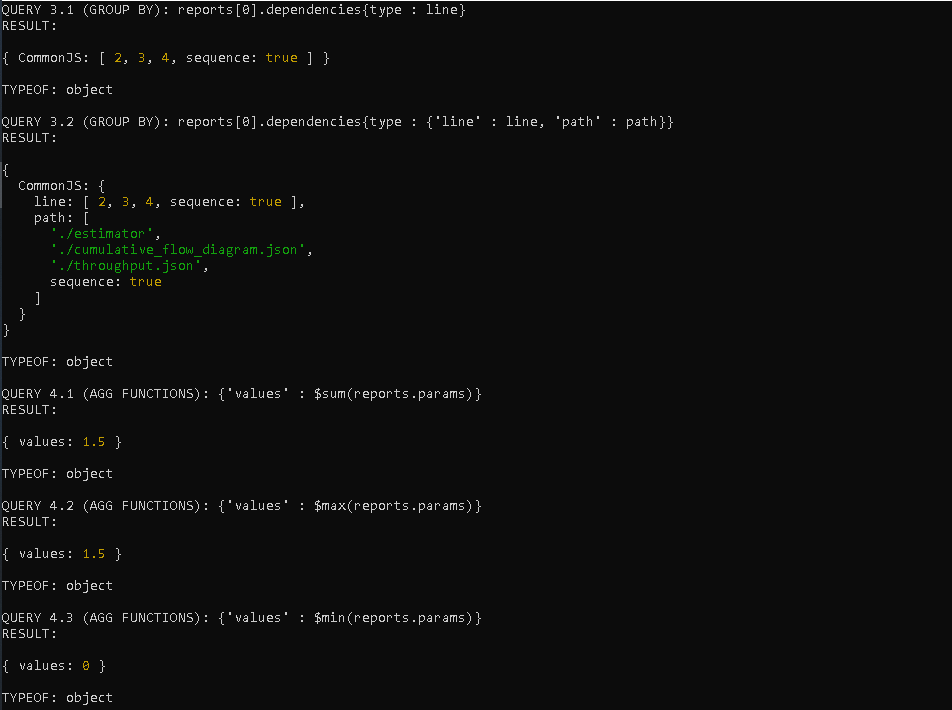
\includegraphics[width=16cm]{JSONata.png}
					\label{figure:Image}
				\end{figure}
		\newpage \subsection{fx - Command-line tool and terminal JSON viewer}
			\subsubsection{Introdução}
				O fx foi desenvolvido para ser semelhante ao jq, porém com algumas interessantes diferenças. O fx possui suporte para a linguagem \textbf{JSONata}, que é uma linguagem de query para arquivos JSON, além disso é possível usar \textbf{JavaScript} para realizar consultas.

				O fx possui dois modos de uso: \textbf{CLI} e \textbf{Interativo}. O modo interativo funciona como o \textbf{VIM}, enquanto o modo CLI é usado como o jq.
			\subsubsection{Sintaxe}
				Considerando o uso da ferramenta, o modo mais relevante é o \textbf{CLI com JSONata}. Dessa forma, basta conhecer a linguagem de query para realizar consultas.
			\subsubsection{Consulta Simples}
				Para obter o atributo “maintainability" do primeiro objeto no array “reports", é possível usar:
\begin{lstlisting}[language=bash]
$ fx Request.json 'jsonata("reports[0].maintainability)"'
\end{lstlisting}
			\subsubsection{Where}
				Para obtermos o objeto “reports" que tem o atributo “params" equivalente a “0", podemos utilizar:
\begin{lstlisting}[language=bash]
$ fx Request.json 'jsonata("reports[params=0]")'
\end{lstlisting}
				
				O reseultado será:
\begin{lstlisting}[language=json,firstnumber=1]
{
  "aggregate": {
    "sloc": {
      "logical": 5,
      "physical": 7
    },
  [...],
  "params": 0,
  "path": "cli.js"
}
\end{lstlisting}
			\subsubsection{Group By}
				Para obtermos todos os atributos “path" do array “dependencies" do primeiro objeto do array “reports" organizados em um array chamado “Caminho", podemos fazer:
\begin{lstlisting}[language=bash]
$ fx Request.json 'jsonata("reports[0].dependencies{'Caminho' : path}")'
\end{lstlisting}

				O resultado será:
\begin{lstlisting}[language=json,firstnumber=1]
{
  "Caminho": [
    "./estimator",
    "./cumulative_flow_diagram.json",
    "./throughput.json"
  ]
}
\end{lstlisting}
			\subsubsection{Join}
				Por trabalhar com um único arquivo JSON, o JSONata não possui suporte para a cláusula Join do SQL (Apesar de ser possível simular).
			\subsubsection{Funções de Agregação}
				JSONata possui suporte nativo para funções de agregação, assim é muito simples utilizar. Por exemplo, podemos obter a soma do atributo “params" de todos os objetos do array “reports":
\begin{lstlisting}[language=bash]
$ fx Request.json 'jsonata("{"values" : $sum(reports.params)}")'
\end{lstlisting}

				O resultado será:
\begin{lstlisting}[language=json,firstnumber=1]
{
  "values": 1.5
}
\end{lstlisting}

				Para que o resultado fosse um objeto JSON, foi necessário usar um \textbf{Group By}.
		\newpage \subsection{emuto - JSON Processor}
			\subsubsection{Introdução}
				O emuto é semelhante ao jx em questão de funcionamento e sintaxe. Pode ser instalado pelo npm usando:
\begin{lstlisting}[language=bash]
$ npm install -g emuto emuto-cli
\end{lstlisting}

				É um projeto de código aberto e possui uma documentação muito bem escrita. É um projeto relativamente menor que o jx, porém igualmente confiável.

				Possui um simulador online presente em \textit{\textbf{https://kantord.github.io/emuto/docs/\\try\_emuto}}.
			\subsubsection{Sintaxe}
				O emuto pode ser utilizado da seguinte forma:
\begin{lstlisting}[language=bash]
$ cat file.json | emuto 'query'
\end{lstlisting}

				Sua linguagem de query é baseada em \textbf{GraphQL}, assim são consideravelmente semelhantes. 

				O emuto não foi projetado para ser uma linguagem exclusivamente de query, e sim uma linguagem de manipulação e processamento de arquivos JSON, em função disso sua sintaxe não é idêntica a GraphQL.
			\subsubsection{Scripts}
				Um diferencial do emuto para outras ferramentas é a possibilidade de criar um script para realizar a consulta em um JSON. Dessa forma, basta criar um arquivo com extensão \textit{.emu} e usar da seguinte forma:
\begin{lstlisting}[language=bash]
$ cat file.json | ./file.emu
\end{lstlisting}

				Como exemplo de um script \textit{.emu} temos:
\begin{lstlisting}
#! emuto -s

$
  | map ($ => $ { commit { message } committer { login } } )
  | map ($ => {
      "committer": $.committer.login,
      "message":   $.commit.message,
    })
\end{lstlisting}
			\subsubsection{Linguagem de Query}
				Sua linguagem de query tem o objetivo de criar uma nova estrutura a partir de um JSON existente. Dessa forma, pode-se dizer que o usuário cria a estrutura final do JSON enquanto o emuto preenche os campos.
			\subsubsection{Consulta Simples}
				Para obter o atributo “loc", basta realizar a seguinte query:
\begin{lstlisting}[language=bash]
$ cat Request.json | emuto '$.loc'
\end{lstlisting}
			\subsubsection{Funções de Agregação}
				Para obtermos, por exemplo, o número de objetos no array “reports", basta executarmos a query:
\begin{lstlisting}[language=bash]
$ cat Request.json | emuto '$ { ...Stats }

where
  $Stats=($=>{
      "Reports Length":($.reports|length)
    })'
\end{lstlisting}

				O resultado será:
\begin{lstlisting}[language=json,firstnumber=1]
{
  "Reports Length": 2
}
\end{lstlisting}
		\newpage \subsection{json-query - Retrieves values from JSON objects for data binding}
			\subsubsection{Introdução}
				O json-query é uma biblioteca JavaScript desenvolvida para extrair informações de JSON e usá-los de maneira nativa. Infelizmente, o projeto não recebe modificações desde 2017. Sua sintaxe é bastante simples e tem o objetivo de lidar mais com o objeto nativo do que com o resultado da query. Dessa forma, o json-query precisa de uma grande quantidade de código pré-definido para obter resultados complexos.
			
			\subsubsection{Linguagem de Query e Exemplos}
				Como exemplo, é possível acessar o projeto disponível na seguinte página: \textbf{\textit{https://\\github.com/GabrielIDSM/JSON-And-Queries/tree/master/Projects/\\json-query Project}}.

				\begin{figure}[H]
					\centering
					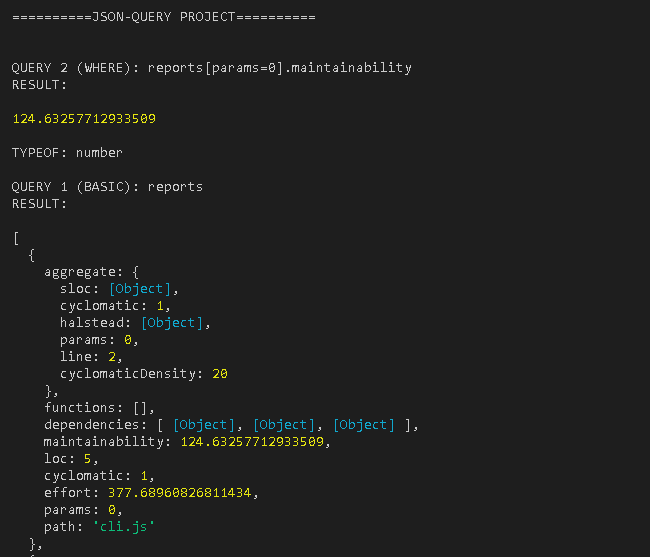
\includegraphics[width=16cm]{json-query.png}
					\label{figure:Image}
				\end{figure}
	\newpage \section{Python}
		\subsection{jello - Filter JSON and JSON Lines data}
			\subsubsection{Introdução}
				O jello foi desenvolvido para ser, resumidamente, \textit{“um jq que utiliza uma query em python"}. Dessa forma, ele possui as mesmas funcionalidades do jq, porém utiliza a sintaxe de Python para realizar consultas.

				Essa ferramenta é relativamente recente, a mais nova de todas as ferramentas citadas. Em função disso, não possui muitos contribuidores. Ela é desenvolvida por \textbf{Kelly Brazil} e é disponibilizada sob a licença do MIT.

				Seu código pode ser encontrado no GitHub na página \textit{\textbf{https://github.com/\\kellyjonbrazil/jello}}.

				Sua instalação pode ser feita via terminal:
\begin{lstlisting}[language=bash]
$ pip3 install jello
\end{lstlisting}

				Para usar o \textit{pip} basta ter o Python instalado.
			\subsubsection{Sintaxe}
				Para executar uma query em um arquivo JSON usando o jello, basta seguir o seguinte padrão:
\begin{lstlisting}[language=bash]
$ cat file.json | jello 'op' 'query'
\end{lstlisting}

				Sua query utiliza da sintaxe pura de \textbf{Python 3}, assim basta conhecer a linguagem para conseguir construir uma query.

				Uma \textit{feature} muito útil do jello é a implementação do módulo \textbf{glom}. O glom é um módulo de manipulação de dados para Python, útil para operações em estruturas aninhadas.

				Para poder usar o glom, é necessário adicionar a seguinte linha no arquivo \textit{.jelloconf.py}:
\begin{lstlisting}
from glom import *
\end{lstlisting}
			\subsubsection{Consulta}
				Apesar de ser uma ferramenta prática, sua linguagem de query possui muitas limitações. Por ser baseada em Python, consultas complexas exigem grande esforço por parte do programador para desenvolver a query.

				Por exemplo, para listar todos os objetos no array “reports" devemos fazer:
\begin{lstlisting}[language=bash]
$ cat Request.json | jello '\
result=[]
for data in _["reports"]:
  result.append(data)
result'
\end{lstlisting}

				\newpage O resultado da query será:
\begin{lstlisting}[language=json,firstnumber=1]
{
  [
    {
      "aggregate": {
      "sloc": {
        "logical": 5,
        "physical": 7
      },
      [...],
      "path": "cli.js"
    },
    {
      "aggregate": {
      "sloc": {
        "logical": 20,
        "physical": 62
      },
      [...],
      "path": "estimator.js"
    }
  ]
}
\end{lstlisting}
	\newpage \section{Lua}
		\subsection{JMESPath.lua}
			\subsubsection{Introdução}
				JMESPath é um projeto desenvolvido por James Saryerwinnie disponibilizado em linguagens como Lua, JavaScript, PHP, Python, Java, Ruby, Go e etc. Para fins práticos, os testes serão feito utilizando a biblioteca \textbf{jmespath.lua}.

				Essa biblioteca tem o objetivo de executar queries em arquivos JSON e obter um novo JSON como resposta. Sua linguagem de query é extremamente complexa e possui suporte para diversos operadores.

				Infelizmente, a última atualização que a ferramenta recebeu foi em 2014. Além disso, não existe suporte para operações de Join e Group By.
			\subsubsection{Linguagem de Query e Exemplos}
				Como exemplo, é possível acessar o projeto disponível na seguinte página: \textbf{\textit{https://\\github.com/GabrielIDSM/JSON-And-Queries/tree/master/Projects/\\JMESPath Project}}.
			\begin{figure}[H]
				\centering
				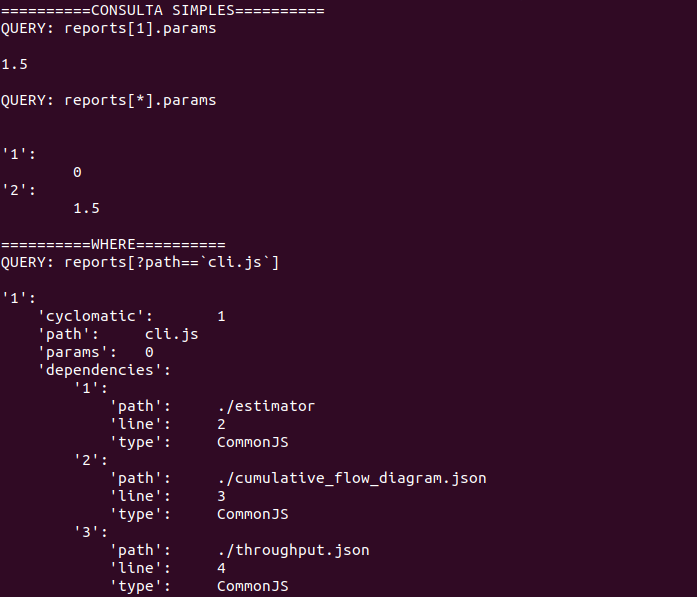
\includegraphics[width=16cm]{jmespath-lua.png}
				\label{figure:Image}
			\end{figure}
	\newpage \section{PHP}
		\subsection{jsonq - A PHP query builder for JSON}
			\subsubsection{Introdução}
				jsonq é uma ferramenta desenvolvida para projetos em PHP para realização de queries em arquivos JSON. É uma ferramenta bastante complexa e possui suporte para as principais operações de query.
			\subsubsection{Linguagem de Query e Exemplos}
				Como exemplo, é possível acessar o projeto disponível na seguinte página: \textbf{\textit{https://\\github.com/GabrielIDSM/JSON-And-Queries/tree/master/Projects/\\jsonq Project}}.
			\begin{figure}[H]
				\centering
				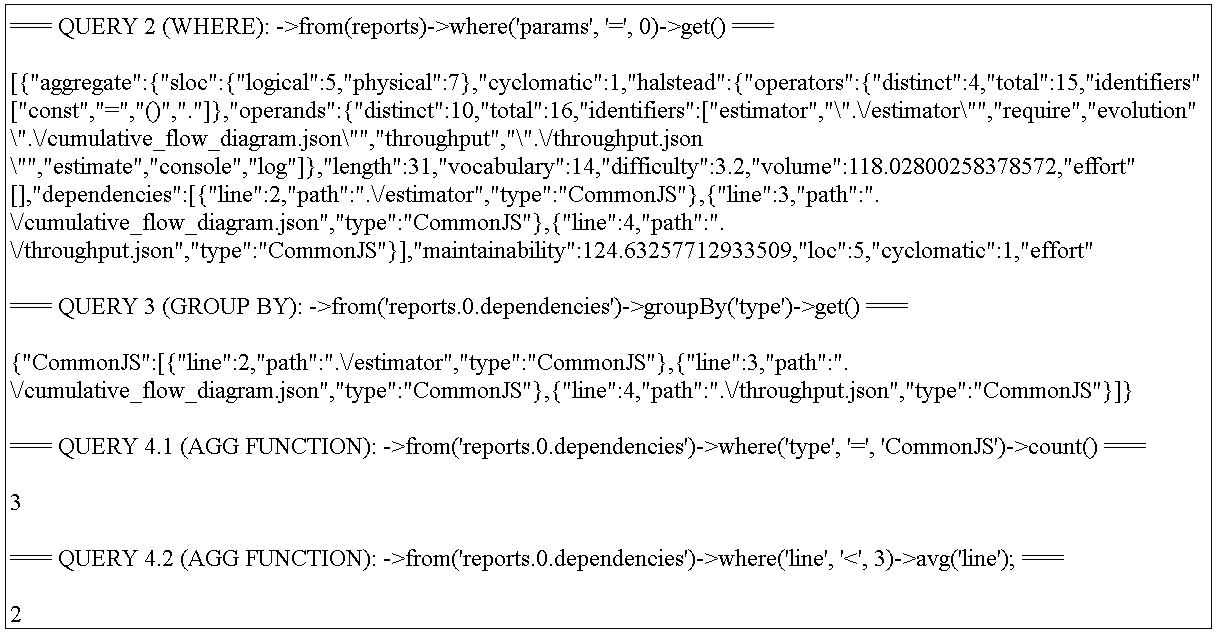
\includegraphics[width=16cm]{jsonq.png}
				\label{figure:Image}
			\end{figure}

	\newpage \section{Go}
		\subsection{dasel - Query, update and convert data structures}
			\subsubsection{Introdução}
				Dasel (de \textit{\textbf{da}ta \textbf{sel}ector}) é uma ferramenta de linha de comando desenvolvida em Go. É um dos projetos com maior suporte da comunidade, onde sua versão mais recente foi publicada já em 2021. Apesar de ser semelhante a ferramenta como o \textbf{jq} e o \textbf{yq}, o dasel possui suporte para I/O para os formatos JSON, YAML, TOML, XML e CSV sem precisar de nenhuma dependência.
			\subsubsection{Consulta Simples}
				Utilizando como exemplo o arquivos Request.json, podemos obter o atributo \textit{changeCost} da seguinte forma:
\begin{lstlisting}[language=bash]
$ dasel -f Request.json '.changeCost'
\end{lstlisting}
				Ou ainda dessa outra forma:
\begin{lstlisting}[language=bash]
$ dasel select -f Request.json -p json -s '.changeCost'
\end{lstlisting}
				Para escolher um item no array \textit{reports} é possível usar:
\begin{lstlisting}[language=bash]
$ dasel select -f Request.json -p json -s '.reports.[0]'
\end{lstlisting}
				Para todos os itens no array deve-se usar:
\begin{lstlisting}[language=bash]
$ dasel select -f Request.json -p json -s '.reports.[*]' -m
\end{lstlisting}
			\subsubsection{Where}
				Para obter o elemento no array que tem o campo \textit{path} igual a \textit{cli.js} temos:
\begin{lstlisting}[language=bash]
$ dasel select -f Request.json -p json -s '.reports.(path=cli.js)'
\end{lstlisting}
				Para obter todos os elementos do array \textit{dependencies} no objeto de index 0 no array \textit{reports} que possuem o campo \textit{type} igual a \textit{CommonJS} temos:
\begin{lstlisting}[language=bash]
$ dasel select -f Request.json -p json -s '.reports.[0]
.dependencies.(type=CommonJS)' -m
\end{lstlisting}
			\subsubsection{Limitações e \textit{Features}}
				Diferente de algumas ferramentas disponíveis, o dasel não possui suporte para operações como \textit{Join} e \textit{Group By}. Contudo, essa ferramenta possui suporte para inserção, remoção e atualização de campos em arquivos de diversos formatos.

				Dessa forma, é uma ferramenta muito útil para \textbf{auxiliar outras ferramentas de query}, já que é possível modificar o arquivo JSON e converter de/para outros formatos.
\end{document}


















